% Options for packages loaded elsewhere
\PassOptionsToPackage{unicode}{hyperref}
\PassOptionsToPackage{hyphens}{url}
\PassOptionsToPackage{dvipsnames,svgnames,x11names}{xcolor}
%
\documentclass[
  letterpaper,
  oneside]{scrbook}

\usepackage{amsmath,amssymb}
\usepackage{iftex}
\ifPDFTeX
  \usepackage[T1]{fontenc}
  \usepackage[utf8]{inputenc}
  \usepackage{textcomp} % provide euro and other symbols
\else % if luatex or xetex
  \usepackage{unicode-math}
  \defaultfontfeatures{Scale=MatchLowercase}
  \defaultfontfeatures[\rmfamily]{Ligatures=TeX,Scale=1}
\fi
\usepackage{lmodern}
\ifPDFTeX\else  
    % xetex/luatex font selection
\fi
% Use upquote if available, for straight quotes in verbatim environments
\IfFileExists{upquote.sty}{\usepackage{upquote}}{}
\IfFileExists{microtype.sty}{% use microtype if available
  \usepackage[]{microtype}
  \UseMicrotypeSet[protrusion]{basicmath} % disable protrusion for tt fonts
}{}
\makeatletter
\@ifundefined{KOMAClassName}{% if non-KOMA class
  \IfFileExists{parskip.sty}{%
    \usepackage{parskip}
  }{% else
    \setlength{\parindent}{0pt}
    \setlength{\parskip}{6pt plus 2pt minus 1pt}}
}{% if KOMA class
  \KOMAoptions{parskip=half}}
\makeatother
\usepackage{xcolor}
\setlength{\emergencystretch}{3em} % prevent overfull lines
\setcounter{secnumdepth}{5}
% Make \paragraph and \subparagraph free-standing
\ifx\paragraph\undefined\else
  \let\oldparagraph\paragraph
  \renewcommand{\paragraph}[1]{\oldparagraph{#1}\mbox{}}
\fi
\ifx\subparagraph\undefined\else
  \let\oldsubparagraph\subparagraph
  \renewcommand{\subparagraph}[1]{\oldsubparagraph{#1}\mbox{}}
\fi


\providecommand{\tightlist}{%
  \setlength{\itemsep}{0pt}\setlength{\parskip}{0pt}}\usepackage{longtable,booktabs,array}
\usepackage{calc} % for calculating minipage widths
% Correct order of tables after \paragraph or \subparagraph
\usepackage{etoolbox}
\makeatletter
\patchcmd\longtable{\par}{\if@noskipsec\mbox{}\fi\par}{}{}
\makeatother
% Allow footnotes in longtable head/foot
\IfFileExists{footnotehyper.sty}{\usepackage{footnotehyper}}{\usepackage{footnote}}
\makesavenoteenv{longtable}
\usepackage{graphicx}
\makeatletter
\def\maxwidth{\ifdim\Gin@nat@width>\linewidth\linewidth\else\Gin@nat@width\fi}
\def\maxheight{\ifdim\Gin@nat@height>\textheight\textheight\else\Gin@nat@height\fi}
\makeatother
% Scale images if necessary, so that they will not overflow the page
% margins by default, and it is still possible to overwrite the defaults
% using explicit options in \includegraphics[width, height, ...]{}
\setkeys{Gin}{width=\maxwidth,height=\maxheight,keepaspectratio}
% Set default figure placement to htbp
\makeatletter
\def\fps@figure{htbp}
\makeatother

\usepackage{makeidx}
\usepackage{fancyhdr}
\usepackage{xcolor}
\usepackage{booktabs}
\usepackage{graphicx}
\makeindex
\pagestyle{fancy}
\fancyhead[LE,RO]{\thepage}
\fancyhead[RE]{\textit{\leftmark}}
\fancyhead[LO]{\textit{\rightmark}}
\makeatletter
\@ifpackageloaded{bookmark}{}{\usepackage{bookmark}}
\makeatother
\makeatletter
\@ifpackageloaded{caption}{}{\usepackage{caption}}
\AtBeginDocument{%
\ifdefined\contentsname
  \renewcommand*\contentsname{Table of contents}
\else
  \newcommand\contentsname{Table of contents}
\fi
\ifdefined\listfigurename
  \renewcommand*\listfigurename{List of Figures}
\else
  \newcommand\listfigurename{List of Figures}
\fi
\ifdefined\listtablename
  \renewcommand*\listtablename{List of Tables}
\else
  \newcommand\listtablename{List of Tables}
\fi
\ifdefined\figurename
  \renewcommand*\figurename{Figure}
\else
  \newcommand\figurename{Figure}
\fi
\ifdefined\tablename
  \renewcommand*\tablename{Table}
\else
  \newcommand\tablename{Table}
\fi
}
\@ifpackageloaded{float}{}{\usepackage{float}}
\floatstyle{ruled}
\@ifundefined{c@chapter}{\newfloat{codelisting}{h}{lop}}{\newfloat{codelisting}{h}{lop}[chapter]}
\floatname{codelisting}{Listing}
\newcommand*\listoflistings{\listof{codelisting}{List of Listings}}
\makeatother
\makeatletter
\makeatother
\makeatletter
\@ifpackageloaded{caption}{}{\usepackage{caption}}
\@ifpackageloaded{subcaption}{}{\usepackage{subcaption}}
\makeatother
\ifLuaTeX
  \usepackage{selnolig}  % disable illegal ligatures
\fi
\usepackage{bookmark}

\IfFileExists{xurl.sty}{\usepackage{xurl}}{} % add URL line breaks if available
\urlstyle{same} % disable monospaced font for URLs
\hypersetup{
  pdftitle={Retrieval Augmented Generation (RAG)},
  pdfauthor={Hamel Husain},
  colorlinks=true,
  linkcolor={blue},
  filecolor={Maroon},
  citecolor={Blue},
  urlcolor={blue},
  pdfcreator={LaTeX via pandoc}}

\title{Retrieval Augmented Generation (RAG)}
\usepackage{etoolbox}
\makeatletter
\providecommand{\subtitle}[1]{% add subtitle to \maketitle
  \apptocmd{\@title}{\par {\large #1 \par}}{}{}
}
\makeatother
\subtitle{From Fundamentals to Advanced Techniques}
\author{Hamel Husain}
\date{2025-08-06}

\begin{document}
\frontmatter
\maketitle

\begin{titlepage}
\centering
\vspace*{3cm}
{\Huge\bfseries Retrieval Augmented Generation (RAG)\par}
\vspace{1cm}
{\Large From Fundamentals to Advanced Techniques\par}
\vspace{2cm}
{\Large Hamel Husain\par}
\vspace{1cm}
{\large \today\par}
\vspace{2cm}
{\large A comprehensive guide to understanding and implementing\\ Retrieval Augmented Generation systems\par}
\end{titlepage}

\renewcommand*\contentsname{Table of contents}
{
\hypersetup{linkcolor=}
\setcounter{tocdepth}{2}
\tableofcontents
}
\mainmatter
\bookmarksetup{startatroot}

\chapter{Introduction}\label{introduction}

\bookmarksetup{startatroot}

\chapter{Retrieval Augmented Generation
(RAG)}\label{retrieval-augmented-generation-rag}

\section{The Future of AI is
Retrieval}\label{the-future-of-ai-is-retrieval}

In the rapidly evolving landscape of artificial intelligence, one
technology stands at the intersection of knowledge and generation:
Retrieval Augmented Generation (RAG). Despite claims that larger context
windows might render it obsolete, RAG continues to be the backbone of
the most powerful AI systems today.

This book takes you on a journey through the world of RAG---from its
fundamental concepts to cutting-edge techniques that are reshaping how
AI systems access and utilize information. RAG isn't just about
extending context windows; it's about finding the \emph{right}
information at the right time.

As large language models continue to advance, the ability to retrieve
relevant information becomes not less important, but more critical. Even
with infinite context, the challenge of finding the needle in the
haystack remains. This is where RAG shines---providing AI systems with
the ability to access and leverage external knowledge beyond their
training data.

In the following chapters, we'll explore:

\begin{itemize}
\tightlist
\item
  Why RAG is far from dead, and in fact, just getting started
\item
  Advanced retrieval techniques that go beyond simple vector similarity
\item
  Evaluation methods to measure and improve RAG system performance
\item
  Reasoning capabilities that allow models to synthesize information
  across sources
\item
  Late interaction approaches that make retrieval more efficient and
  effective
\item
  A comprehensive map of the RAG landscape to guide your implementation
\end{itemize}

Whether you're building your first RAG system or looking to optimize an
existing one, this book provides the insights and techniques you need to
harness the full power of Retrieval Augmented Generation.

\part{Foundations}

\chapter{Stop Saying RAG Is Dead}\label{stop-saying-rag-is-dead}

\chapter{Stop Saying RAG Is Dead}\label{stop-saying-rag-is-dead-1}

\includegraphics{chapters/../rag_dead.png}

Why the future of RAG lies in better retrieval, not bigger context
windows.

By Hamel Husain and Ben Clavié

I've been seeing a lot of posts lately claiming that RAG is dead or will
be obsolete soon due to larger context windows. This is a
misunderstanding of what RAG is and why it's valuable.

RAG isn't just about extending context windows - it's about
\textbf{relevant} information retrieval. Even with infinite context, you
still need to find the right information.

\section{The Real Problem: Retrieval
Quality}\label{the-real-problem-retrieval-quality}

The core challenge in RAG is finding the most relevant information for a
given query. This remains true regardless of context window size.

Consider these scenarios:

\begin{enumerate}
\def\labelenumi{\arabic{enumi}.}
\tightlist
\item
  \textbf{Small context window + poor retrieval}: You can only fit a few
  documents, and they're not even the right ones.
\item
  \textbf{Large context window + poor retrieval}: You can fit more
  documents, but most are irrelevant noise.
\item
  \textbf{Any context window + good retrieval}: You get precisely the
  information needed to answer the query.
\end{enumerate}

The third scenario is always superior, regardless of context size.

\section{Why Bigger Context Windows Aren't
Enough}\label{why-bigger-context-windows-arent-enough}

Larger context windows don't solve the fundamental problem of finding
the right information. In fact, they can make things worse by:

\begin{enumerate}
\def\labelenumi{\arabic{enumi}.}
\tightlist
\item
  \textbf{Increasing noise}: More irrelevant information can confuse the
  model
\item
  \textbf{Raising costs}: Processing larger contexts is more expensive
\item
  \textbf{Reducing performance}: Models often perform worse with too
  much irrelevant context
\end{enumerate}

\section{The Future of RAG}\label{the-future-of-rag}

The future of RAG isn't about cramming more documents into context -
it's about:

\begin{enumerate}
\def\labelenumi{\arabic{enumi}.}
\tightlist
\item
  \textbf{Better retrieval}: Finding exactly the right information
\item
  \textbf{Reasoning over documents}: Synthesizing information across
  sources
\item
  \textbf{Late interaction}: Deferring expensive operations until needed
\item
  \textbf{Hybrid approaches}: Combining dense and sparse retrieval
  methods
\end{enumerate}

\section{Conclusion}\label{conclusion}

RAG isn't dying - it's evolving. The focus is shifting from ``how much
context can we fit?'' to ``how can we find exactly the right
information?''

Even with infinite context windows, you'd still need effective retrieval
to find the needle in the haystack.

So no, RAG isn't dead. It's just getting started.

\chapter{I don't use RAG, I just retrieve
documents}\label{i-dont-use-rag-i-just-retrieve-documents}

\chapter{I don't use RAG, I just retrieve
documents}\label{i-dont-use-rag-i-just-retrieve-documents-1}

As part of our \href{https://bit.ly/evals-ai}{LLM Evals course}, I
hosted \href{https://ben.clavie.eu/}{Benjamin Clavié} to kick off a
5-part mini-series on evaluating and optimizing RAG. Ben is a retrieval
researcher who has built widely used tools like
\href{https://github.com/answerdotai/ragatouille}{RAGatouille} and
\href{https://github.com/answerdotai/rerankers}{rerankers} among other
things. His talk focused on important developments in RAG and where you
should be paying attention (late-interaction, reasoning, evals,
multimodal, etc.).

Below is an annotated version of the presentation, with timestamped
links for each slide.

Watch the full presentation on YouTube

\section{Introduction}\label{introduction-1}

\includegraphics{chapters/../p1-images/slide_1.png}

Ben starts by introducing himself and his background in retrieval
research. He's the founder of \href{https://answer.ai/}{Answer.ai}, a
company focused on building better retrieval systems.

\section{The State of RAG}\label{the-state-of-rag}

\includegraphics{chapters/../p1-images/slide_2.png}

Ben discusses the current state of RAG and how it's evolved over the
past year. He notes that while RAG has become more popular, there's
still a lot of confusion about what it is and how to use it effectively.

\section{RAG is Not Just About Context
Windows}\label{rag-is-not-just-about-context-windows}

\includegraphics{chapters/../p1-images/slide_3.png}

A common misconception is that RAG is just about extending context
windows. Ben emphasizes that RAG is about finding the most relevant
information for a given query, regardless of context window size.

\section{The Evolution of Retrieval}\label{the-evolution-of-retrieval}

\includegraphics{chapters/../p1-images/slide_4.png}

Ben traces the evolution of retrieval from simple keyword matching to
modern neural approaches. He highlights how retrieval has become more
sophisticated over time.

\section{Dense Retrieval}\label{dense-retrieval}

\includegraphics{chapters/../p1-images/slide_5.png}

Dense retrieval involves encoding queries and documents into dense
vector representations and finding the most similar documents to a
query. This approach has become the standard for modern retrieval
systems.

\section{Hybrid Retrieval}\label{hybrid-retrieval}

\includegraphics{chapters/../p1-images/slide_6.png}

Hybrid retrieval combines multiple retrieval methods (e.g., dense and
sparse) to get the best of both worlds. Ben discusses how hybrid
approaches can improve retrieval quality.

\section{Re-ranking}\label{re-ranking}

\includegraphics{chapters/../p1-images/slide_7.png}

Re-ranking involves taking the results from a retrieval system and
re-ordering them based on a more sophisticated model. This can
significantly improve retrieval quality.

\section{Late Interaction}\label{late-interaction}

\includegraphics{chapters/../p1-images/slide_8.png}

Late interaction defers expensive operations until they're needed. Ben
explains how this approach can make retrieval more efficient.

\section{Reasoning Over Documents}\label{reasoning-over-documents}

\includegraphics{chapters/../p1-images/slide_9.png}

Reasoning over documents involves synthesizing information across
multiple sources. Ben discusses how this can lead to more accurate and
comprehensive answers.

\section{Evaluating RAG Systems}\label{evaluating-rag-systems}

\includegraphics{chapters/../p1-images/slide_10.png}

Ben emphasizes the importance of evaluating RAG systems properly. He
discusses various metrics and approaches for measuring retrieval
quality.

\section{The Future of RAG}\label{the-future-of-rag-1}

\includegraphics{chapters/../p1-images/slide_11.png}

Ben concludes by discussing the future of RAG and where he sees the
field heading. He emphasizes that RAG will continue to evolve and
improve as retrieval methods become more sophisticated.

\section{Q\&A}\label{qa}

The presentation ends with a Q\&A session where Ben answers questions
from the audience about RAG, retrieval, and related topics.

\part{Advanced Techniques}

\chapter{Evaluating RAG Systems}\label{evaluating-rag-systems-1}

\chapter{Evaluating RAG Systems}\label{evaluating-rag-systems-2}

In this chapter, we'll explore how to evaluate RAG systems effectively.
Evaluation is crucial for understanding the performance of your RAG
system and identifying areas for improvement.

\section{Introduction to RAG
Evaluation}\label{introduction-to-rag-evaluation}

\includegraphics{chapters/../p2-images/slide_1.png}

Evaluation is a critical component of building effective RAG systems.
Without proper evaluation, it's difficult to know if your system is
actually improving or if changes are making things worse.

\section{Types of Evaluation Metrics}\label{types-of-evaluation-metrics}

\includegraphics{chapters/../p2-images/slide_2.png}

There are several types of evaluation metrics for RAG systems:

\begin{enumerate}
\def\labelenumi{\arabic{enumi}.}
\tightlist
\item
  \textbf{Retrieval metrics}: Measure how well the system retrieves
  relevant documents
\item
  \textbf{Generation metrics}: Measure the quality of the generated
  responses
\item
  \textbf{End-to-end metrics}: Measure the overall performance of the
  system
\end{enumerate}

\section{Retrieval Metrics}\label{retrieval-metrics}

\includegraphics{chapters/../p2-images/slide_3.png}

Retrieval metrics focus on how well the system retrieves relevant
documents. Common metrics include:

\begin{itemize}
\tightlist
\item
  \textbf{Precision}: The fraction of retrieved documents that are
  relevant
\item
  \textbf{Recall}: The fraction of relevant documents that are retrieved
\item
  \textbf{F1 Score}: The harmonic mean of precision and recall
\item
  \textbf{Mean Average Precision (MAP)}: The mean of average precision
  scores for each query
\item
  \textbf{Normalized Discounted Cumulative Gain (NDCG)}: Measures the
  ranking quality of the retrieved documents
\end{itemize}

\section{Generation Metrics}\label{generation-metrics}

\includegraphics{chapters/../p2-images/slide_4.png}

Generation metrics focus on the quality of the generated responses.
Common metrics include:

\begin{itemize}
\tightlist
\item
  \textbf{BLEU}: Measures the similarity between the generated text and
  reference text
\item
  \textbf{ROUGE}: Measures the overlap of n-grams between the generated
  text and reference text
\item
  \textbf{BERTScore}: Measures the semantic similarity between the
  generated text and reference text
\item
  \textbf{Faithfulness}: Measures how well the generated text aligns
  with the retrieved documents
\item
  \textbf{Relevance}: Measures how well the generated text addresses the
  query
\end{itemize}

\section{End-to-End Metrics}\label{end-to-end-metrics}

\includegraphics{chapters/../p2-images/slide_5.png}

End-to-end metrics measure the overall performance of the system. These
metrics often involve human evaluation or automated metrics that
correlate well with human judgment.

\section{Challenges in RAG
Evaluation}\label{challenges-in-rag-evaluation}

\includegraphics{chapters/../p2-images/slide_6.png}

Evaluating RAG systems comes with several challenges:

\begin{enumerate}
\def\labelenumi{\arabic{enumi}.}
\tightlist
\item
  \textbf{Subjectivity}: Different people may have different opinions on
  what constitutes a good response
\item
  \textbf{Context dependence}: The quality of a response may depend on
  the context in which it's used
\item
  \textbf{Multiple correct answers}: There may be multiple valid ways to
  answer a query
\item
  \textbf{Lack of standardized benchmarks}: There are few standardized
  benchmarks for RAG evaluation
\end{enumerate}

\section{Building an Evaluation
Pipeline}\label{building-an-evaluation-pipeline}

\includegraphics{chapters/../p2-images/slide_7.png}

Building an effective evaluation pipeline involves:

\begin{enumerate}
\def\labelenumi{\arabic{enumi}.}
\tightlist
\item
  \textbf{Defining clear metrics}: Choose metrics that align with your
  goals
\item
  \textbf{Creating a test set}: Build a diverse and representative test
  set
\item
  \textbf{Automating evaluation}: Set up automated evaluation to run
  regularly
\item
  \textbf{Human evaluation}: Incorporate human evaluation for subjective
  aspects
\item
  \textbf{Continuous improvement}: Use evaluation results to guide
  system improvements
\end{enumerate}

\section{Case Study: Evaluating a RAG
System}\label{case-study-evaluating-a-rag-system}

\includegraphics{chapters/../p2-images/slide_8.png}

Let's walk through a case study of evaluating a RAG system:

\begin{enumerate}
\def\labelenumi{\arabic{enumi}.}
\tightlist
\item
  \textbf{Define metrics}: We'll use precision@k for retrieval and a
  combination of relevance and faithfulness for generation
\item
  \textbf{Create test set}: We'll create a test set of 100 diverse
  queries
\item
  \textbf{Run evaluation}: We'll evaluate the system on the test set
\item
  \textbf{Analyze results}: We'll analyze the results to identify
  strengths and weaknesses
\item
  \textbf{Make improvements}: We'll make targeted improvements based on
  the analysis
\end{enumerate}

\section{Conclusion}\label{conclusion-1}

\includegraphics{chapters/../p2-images/slide_9.png}

Evaluation is a crucial component of building effective RAG systems. By
using a combination of retrieval, generation, and end-to-end metrics,
you can gain a comprehensive understanding of your system's performance
and identify areas for improvement.

Remember that evaluation should be an ongoing process, not a one-time
activity. Regularly evaluating your system as you make changes will help
ensure that you're moving in the right direction.

\chapter{Reasoning in RAG Systems}\label{reasoning-in-rag-systems}

\chapter{Reasoning in RAG Systems}\label{reasoning-in-rag-systems-1}

In this chapter, we'll explore the role of reasoning in RAG systems and
how it can improve the quality of generated responses.

\section{Introduction to Reasoning in
RAG}\label{introduction-to-reasoning-in-rag}

\includegraphics{chapters/../p3-images/slide_1.png}

Reasoning is a critical component of advanced RAG systems. It involves
synthesizing information across multiple sources and drawing logical
conclusions based on the retrieved information.

\section{Why Reasoning Matters}\label{why-reasoning-matters}

\includegraphics{chapters/../p3-images/slide_2.png}

Reasoning matters in RAG systems for several reasons:

\begin{enumerate}
\def\labelenumi{\arabic{enumi}.}
\tightlist
\item
  \textbf{Complex queries}: Many queries require reasoning across
  multiple pieces of information
\item
  \textbf{Inconsistent information}: Retrieved documents may contain
  conflicting information that needs to be reconciled
\item
  \textbf{Implicit knowledge}: Some queries require drawing on implicit
  knowledge not explicitly stated in the documents
\item
  \textbf{Multi-hop reasoning}: Some queries require multiple steps of
  reasoning to arrive at an answer
\end{enumerate}

\section{Types of Reasoning}\label{types-of-reasoning}

\includegraphics{chapters/../p3-images/slide_3.png}

There are several types of reasoning that can be incorporated into RAG
systems:

\begin{enumerate}
\def\labelenumi{\arabic{enumi}.}
\tightlist
\item
  \textbf{Deductive reasoning}: Drawing logical conclusions from
  premises
\item
  \textbf{Inductive reasoning}: Making generalizations based on specific
  examples
\item
  \textbf{Abductive reasoning}: Forming the most likely explanation for
  an observation
\item
  \textbf{Analogical reasoning}: Drawing parallels between similar
  situations
\item
  \textbf{Causal reasoning}: Understanding cause-and-effect
  relationships
\end{enumerate}

\section{Implementing Reasoning in
RAG}\label{implementing-reasoning-in-rag}

\includegraphics{chapters/../p3-images/slide_4.png}

There are several approaches to implementing reasoning in RAG systems:

\begin{enumerate}
\def\labelenumi{\arabic{enumi}.}
\tightlist
\item
  \textbf{Chain-of-thought prompting}: Guiding the model through a
  step-by-step reasoning process
\item
  \textbf{Self-consistency}: Generating multiple reasoning paths and
  selecting the most consistent one
\item
  \textbf{Tree-of-thought}: Exploring multiple reasoning paths in a
  tree-like structure
\item
  \textbf{Reasoning over retrieved documents}: Explicitly reasoning over
  the content of retrieved documents
\end{enumerate}

\section{Chain-of-Thought Prompting}\label{chain-of-thought-prompting}

\includegraphics{chapters/../p3-images/slide_5.png}

Chain-of-thought prompting involves guiding the model through a
step-by-step reasoning process. This can be done by:

\begin{enumerate}
\def\labelenumi{\arabic{enumi}.}
\tightlist
\item
  \textbf{Explicit instructions}: Telling the model to ``think step by
  step''
\item
  \textbf{Few-shot examples}: Providing examples of step-by-step
  reasoning
\item
  \textbf{Structured prompts}: Using a structured format to guide the
  reasoning process
\end{enumerate}

\section{Self-Consistency}\label{self-consistency}

\includegraphics{chapters/../p3-images/slide_6.png}

Self-consistency involves generating multiple reasoning paths and
selecting the most consistent one. This can improve the reliability of
the reasoning process.

\section{Tree-of-Thought}\label{tree-of-thought}

\includegraphics{chapters/../p3-images/slide_7.png}

Tree-of-thought involves exploring multiple reasoning paths in a
tree-like structure. This allows the model to consider different
approaches to solving a problem.

\section{Reasoning Over Retrieved
Documents}\label{reasoning-over-retrieved-documents}

\includegraphics{chapters/../p3-images/slide_8.png}

Reasoning over retrieved documents involves explicitly reasoning over
the content of retrieved documents. This can be done by:

\begin{enumerate}
\def\labelenumi{\arabic{enumi}.}
\tightlist
\item
  \textbf{Document-level reasoning}: Reasoning over each document
  individually
\item
  \textbf{Cross-document reasoning}: Reasoning across multiple documents
\item
  \textbf{Document-query reasoning}: Reasoning about the relationship
  between the query and the documents
\end{enumerate}

\section{Case Study: Implementing Reasoning in a RAG
System}\label{case-study-implementing-reasoning-in-a-rag-system}

\includegraphics{chapters/../p3-images/slide_9.png}

Let's walk through a case study of implementing reasoning in a RAG
system:

\begin{enumerate}
\def\labelenumi{\arabic{enumi}.}
\tightlist
\item
  \textbf{Identify reasoning needs}: Determine what types of reasoning
  are needed for your use case
\item
  \textbf{Choose an approach}: Select an appropriate reasoning approach
  (e.g., chain-of-thought)
\item
  \textbf{Implement the approach}: Integrate the reasoning approach into
  your RAG system
\item
  \textbf{Evaluate the results}: Measure the impact of reasoning on
  system performance
\item
  \textbf{Iterate and improve}: Refine the reasoning approach based on
  evaluation results
\end{enumerate}

\section{Challenges in Implementing
Reasoning}\label{challenges-in-implementing-reasoning}

\includegraphics{chapters/../p3-images/slide_10.png}

Implementing reasoning in RAG systems comes with several challenges:

\begin{enumerate}
\def\labelenumi{\arabic{enumi}.}
\tightlist
\item
  \textbf{Computational cost}: Reasoning can be computationally
  expensive
\item
  \textbf{Error propagation}: Errors in reasoning can propagate through
  the system
\item
  \textbf{Balancing depth and breadth}: Finding the right balance
  between deep reasoning and broad coverage
\item
  \textbf{Evaluating reasoning quality}: It can be difficult to evaluate
  the quality of reasoning
\end{enumerate}

\section{Future Directions}\label{future-directions}

\includegraphics{chapters/../p3-images/slide_11.png}

The field of reasoning in RAG is rapidly evolving. Future directions
include:

\begin{enumerate}
\def\labelenumi{\arabic{enumi}.}
\tightlist
\item
  \textbf{More efficient reasoning}: Developing more computationally
  efficient reasoning approaches
\item
  \textbf{Multi-modal reasoning}: Reasoning across different modalities
  (text, images, etc.)
\item
  \textbf{Personalized reasoning}: Adapting reasoning to individual user
  needs and preferences
\item
  \textbf{Explainable reasoning}: Making reasoning processes more
  transparent and explainable
\end{enumerate}

\section{Conclusion}\label{conclusion-2}

\includegraphics{chapters/../p3-images/slide_12.png}

Reasoning is a critical component of advanced RAG systems. By
incorporating reasoning into your RAG system, you can improve the
quality and reliability of generated responses, especially for complex
queries that require synthesizing information across multiple sources.

As the field continues to evolve, we can expect to see more
sophisticated reasoning approaches that further enhance the capabilities
of RAG systems.

\chapter{Late Interaction in RAG
Systems}\label{late-interaction-in-rag-systems}

\chapter{Late Interaction in RAG
Systems}\label{late-interaction-in-rag-systems-1}

In this chapter, we'll explore the concept of late interaction in RAG
systems and how it can improve retrieval efficiency and effectiveness.

\section{Introduction to Late
Interaction}\label{introduction-to-late-interaction}

\includegraphics{chapters/../p4-images/slide_1.png}

Late interaction is an approach to retrieval that defers expensive
operations until they're needed. This can make retrieval more efficient
and effective.

\section{Traditional vs.~Late Interaction
Retrieval}\label{traditional-vs.-late-interaction-retrieval}

\includegraphics{chapters/../p4-images/slide_2.png}

In traditional retrieval, queries and documents are encoded into dense
vectors, and similarity is computed between these vectors. This approach
has limitations:

\begin{enumerate}
\def\labelenumi{\arabic{enumi}.}
\tightlist
\item
  \textbf{Information loss}: Encoding queries and documents into
  fixed-size vectors can lose information
\item
  \textbf{Computational cost}: Computing dense vectors for all documents
  can be expensive
\item
  \textbf{Limited expressiveness}: The similarity function is limited to
  vector similarity
\end{enumerate}

Late interaction addresses these limitations by deferring the
interaction between queries and documents until retrieval time.

\section{How Late Interaction Works}\label{how-late-interaction-works}

\includegraphics{chapters/../p4-images/slide_3.png}

Late interaction works by:

\begin{enumerate}
\def\labelenumi{\arabic{enumi}.}
\tightlist
\item
  \textbf{Encoding tokens}: Instead of encoding entire documents, encode
  individual tokens
\item
  \textbf{Computing token-level similarity}: Compute similarity between
  query tokens and document tokens
\item
  \textbf{Aggregating similarities}: Aggregate token-level similarities
  to get document-level similarity
\end{enumerate}

This approach preserves more information and allows for more expressive
similarity functions.

\section{Colbert: A Late Interaction
Model}\label{colbert-a-late-interaction-model}

\includegraphics{chapters/../p4-images/slide_4.png}

Colbert is a popular late interaction model. It works by:

\begin{enumerate}
\def\labelenumi{\arabic{enumi}.}
\tightlist
\item
  \textbf{Encoding tokens}: Encode query and document tokens using a
  transformer model
\item
  \textbf{Computing token-level similarity}: Compute the maximum
  similarity between each query token and all document tokens
\item
  \textbf{Aggregating similarities}: Sum the maximum similarities to get
  the document score
\end{enumerate}

\section{Benefits of Late
Interaction}\label{benefits-of-late-interaction}

\includegraphics{chapters/../p4-images/slide_5.png}

Late interaction offers several benefits:

\begin{enumerate}
\def\labelenumi{\arabic{enumi}.}
\tightlist
\item
  \textbf{Improved retrieval quality}: By preserving more information,
  late interaction can improve retrieval quality
\item
  \textbf{More expressive similarity}: Late interaction allows for more
  expressive similarity functions
\item
  \textbf{Better handling of long documents}: Late interaction can
  better handle long documents by operating at the token level
\item
  \textbf{Interpretability}: Token-level interactions can provide
  insights into why a document was retrieved
\end{enumerate}

\section{Challenges of Late
Interaction}\label{challenges-of-late-interaction}

\includegraphics{chapters/../p4-images/slide_6.png}

Late interaction also comes with challenges:

\begin{enumerate}
\def\labelenumi{\arabic{enumi}.}
\tightlist
\item
  \textbf{Computational cost}: Computing token-level similarities can be
  more expensive than vector similarity
\item
  \textbf{Storage requirements}: Storing token-level representations can
  require more storage
\item
  \textbf{Implementation complexity}: Implementing late interaction can
  be more complex than traditional retrieval
\end{enumerate}

\section{Optimizing Late Interaction}\label{optimizing-late-interaction}

\includegraphics{chapters/../p4-images/slide_7.png}

There are several approaches to optimizing late interaction:

\begin{enumerate}
\def\labelenumi{\arabic{enumi}.}
\tightlist
\item
  \textbf{Pruning}: Remove low-importance tokens to reduce computation
\item
  \textbf{Quantization}: Reduce the precision of token representations
  to save storage
\item
  \textbf{Caching}: Cache token representations to avoid recomputation
\item
  \textbf{Parallel computation}: Leverage parallel computation to speed
  up token-level similarity
\end{enumerate}

\section{Case Study: Implementing Late
Interaction}\label{case-study-implementing-late-interaction}

\includegraphics{chapters/../p4-images/slide_8.png}

Let's walk through a case study of implementing late interaction in a
RAG system:

\begin{enumerate}
\def\labelenumi{\arabic{enumi}.}
\tightlist
\item
  \textbf{Choose a model}: Select a late interaction model (e.g.,
  Colbert)
\item
  \textbf{Preprocess documents}: Encode document tokens and store the
  representations
\item
  \textbf{Implement retrieval}: Implement token-level similarity
  computation and aggregation
\item
  \textbf{Optimize for efficiency}: Apply optimization techniques to
  improve efficiency
\item
  \textbf{Evaluate performance}: Measure the impact of late interaction
  on retrieval quality and efficiency
\end{enumerate}

\section{Future Directions}\label{future-directions-1}

\includegraphics{chapters/../p4-images/slide_9.png}

The field of late interaction is rapidly evolving. Future directions
include:

\begin{enumerate}
\def\labelenumi{\arabic{enumi}.}
\tightlist
\item
  \textbf{More efficient models}: Developing more computationally
  efficient late interaction models
\item
  \textbf{Multi-modal late interaction}: Extending late interaction to
  multi-modal retrieval
\item
  \textbf{Hybrid approaches}: Combining late interaction with other
  retrieval approaches
\item
  \textbf{End-to-end optimization}: Optimizing late interaction models
  end-to-end for specific tasks
\end{enumerate}

\section{Conclusion}\label{conclusion-3}

\includegraphics{chapters/../p4-images/slide_10.png}

Late interaction is a powerful approach to retrieval that can improve
both efficiency and effectiveness. By deferring expensive operations
until they're needed and operating at the token level, late interaction
preserves more information and allows for more expressive similarity
functions.

As the field continues to evolve, we can expect to see more
sophisticated late interaction models that further enhance the
capabilities of RAG systems.

\chapter{The RAG Map: A Comprehensive
Guide}\label{the-rag-map-a-comprehensive-guide}

\chapter{The RAG Map: A Comprehensive
Guide}\label{the-rag-map-a-comprehensive-guide-1}

In this chapter, we'll explore the RAG Map, a comprehensive guide to the
various components and techniques in Retrieval Augmented Generation.

\section{Introduction to the RAG Map}\label{introduction-to-the-rag-map}

\includegraphics{chapters/../p5-images/slide_1.png}

The RAG Map provides a comprehensive overview of the various components
and techniques in Retrieval Augmented Generation. It serves as a guide
for understanding the RAG landscape and making informed decisions about
which approaches to use.

\section{The Core Components of RAG}\label{the-core-components-of-rag}

\includegraphics{chapters/../p5-images/slide_2.png}

The RAG Map identifies several core components of RAG systems:

\begin{enumerate}
\def\labelenumi{\arabic{enumi}.}
\tightlist
\item
  \textbf{Document processing}: Preparing documents for retrieval
\item
  \textbf{Retrieval}: Finding relevant documents for a query
\item
  \textbf{Generation}: Generating responses based on retrieved documents
\item
  \textbf{Evaluation}: Measuring the performance of the RAG system
\end{enumerate}

\section{Document Processing}\label{document-processing}

\includegraphics{chapters/../p5-images/slide_3.png}

Document processing involves preparing documents for retrieval. This
includes:

\begin{enumerate}
\def\labelenumi{\arabic{enumi}.}
\tightlist
\item
  \textbf{Chunking}: Splitting documents into smaller pieces
\item
  \textbf{Embedding}: Converting text into vector representations
\item
  \textbf{Indexing}: Organizing documents for efficient retrieval
\item
  \textbf{Metadata}: Adding additional information to documents
\end{enumerate}

\section{Retrieval Approaches}\label{retrieval-approaches}

\includegraphics{chapters/../p5-images/slide_4.png}

The RAG Map identifies several retrieval approaches:

\begin{enumerate}
\def\labelenumi{\arabic{enumi}.}
\tightlist
\item
  \textbf{Dense retrieval}: Using dense vector representations for
  retrieval
\item
  \textbf{Sparse retrieval}: Using sparse vector representations (e.g.,
  BM25)
\item
  \textbf{Hybrid retrieval}: Combining dense and sparse approaches
\item
  \textbf{Late interaction}: Deferring expensive operations until needed
\item
  \textbf{Multi-modal retrieval}: Retrieving across different modalities
  (text, images, etc.)
\end{enumerate}

\section{Generation Approaches}\label{generation-approaches}

\includegraphics{chapters/../p5-images/slide_5.png}

The RAG Map identifies several generation approaches:

\begin{enumerate}
\def\labelenumi{\arabic{enumi}.}
\tightlist
\item
  \textbf{Standard generation}: Generating responses based on retrieved
  documents
\item
  \textbf{Chain-of-thought}: Guiding the model through a step-by-step
  reasoning process
\item
  \textbf{Self-consistency}: Generating multiple responses and selecting
  the most consistent one
\item
  \textbf{Tree-of-thought}: Exploring multiple reasoning paths in a
  tree-like structure
\item
  \textbf{Reasoning over documents}: Explicitly reasoning over the
  content of retrieved documents
\end{enumerate}

\section{Evaluation Approaches}\label{evaluation-approaches}

\includegraphics{chapters/../p5-images/slide_6.png}

The RAG Map identifies several evaluation approaches:

\begin{enumerate}
\def\labelenumi{\arabic{enumi}.}
\tightlist
\item
  \textbf{Retrieval metrics}: Measuring retrieval quality (e.g.,
  precision, recall)
\item
  \textbf{Generation metrics}: Measuring generation quality (e.g., BLEU,
  ROUGE)
\item
  \textbf{End-to-end metrics}: Measuring overall system performance
\item
  \textbf{Human evaluation}: Using human judges to evaluate system
  performance
\item
  \textbf{Automated evaluation}: Using automated metrics that correlate
  with human judgment
\end{enumerate}

\section{Advanced RAG Techniques}\label{advanced-rag-techniques}

\includegraphics{chapters/../p5-images/slide_7.png}

The RAG Map also covers advanced RAG techniques:

\begin{enumerate}
\def\labelenumi{\arabic{enumi}.}
\tightlist
\item
  \textbf{Query expansion}: Expanding queries to improve retrieval
\item
  \textbf{Document reranking}: Reordering retrieved documents based on
  relevance
\item
  \textbf{Adaptive retrieval}: Adjusting retrieval based on the query
\item
  \textbf{Multi-step retrieval}: Retrieving documents in multiple steps
\item
  \textbf{Personalized RAG}: Adapting RAG to individual user needs
\end{enumerate}

\section{Navigating the RAG Map}\label{navigating-the-rag-map}

\includegraphics{chapters/../p5-images/slide_8.png}

The RAG Map can be used to navigate the RAG landscape and make informed
decisions about which approaches to use. When navigating the RAG Map,
consider:

\begin{enumerate}
\def\labelenumi{\arabic{enumi}.}
\tightlist
\item
  \textbf{Your use case}: Different approaches may be more suitable for
  different use cases
\item
  \textbf{Resource constraints}: Some approaches may require more
  computational resources
\item
  \textbf{Performance requirements}: Different approaches may offer
  different trade-offs between quality and efficiency
\item
  \textbf{Implementation complexity}: Some approaches may be more
  complex to implement
\end{enumerate}

\section{Case Study: Using the RAG
Map}\label{case-study-using-the-rag-map}

\includegraphics{chapters/../p5-images/slide_9.png}

Let's walk through a case study of using the RAG Map to design a RAG
system:

\begin{enumerate}
\def\labelenumi{\arabic{enumi}.}
\tightlist
\item
  \textbf{Define requirements}: Identify the requirements for your RAG
  system
\item
  \textbf{Explore options}: Use the RAG Map to explore different
  approaches
\item
  \textbf{Make trade-offs}: Consider the trade-offs between different
  approaches
\item
  \textbf{Design the system}: Design a RAG system based on your
  exploration
\item
  \textbf{Implement and evaluate}: Implement the system and evaluate its
  performance
\end{enumerate}

\section{Future Directions}\label{future-directions-2}

\includegraphics{chapters/../p5-images/slide_10.png}

The RAG Map will continue to evolve as the field of RAG advances. Future
directions include:

\begin{enumerate}
\def\labelenumi{\arabic{enumi}.}
\tightlist
\item
  \textbf{New retrieval approaches}: Developing more effective and
  efficient retrieval approaches
\item
  \textbf{New generation approaches}: Developing more sophisticated
  generation approaches
\item
  \textbf{New evaluation approaches}: Developing better ways to evaluate
  RAG systems
\item
  \textbf{Integration with other techniques}: Integrating RAG with other
  AI techniques
\item
  \textbf{Domain-specific RAG}: Adapting RAG to specific domains and use
  cases
\end{enumerate}

\section{Conclusion}\label{conclusion-4}

\includegraphics{chapters/../p5-images/slide_11.png}

The RAG Map provides a comprehensive guide to the various components and
techniques in Retrieval Augmented Generation. By understanding the RAG
landscape, you can make informed decisions about which approaches to use
for your specific use case.

As the field continues to evolve, the RAG Map will be updated to reflect
new developments and best practices.


\backmatter

\end{document}
